% !TeX root = ../main.tex
\documentclass[class=article]{standalone}

\begin{document}
\section*{Question 1}

\subsection*{(a)}

\begin{center}
  \begin{tabular}{|rcl|rcl|}
      \hline
      \multicolumn{3}{|c}{\bf Productions} &
      \multicolumn{3}{|c|}{\bf Règles Sémantiques} \\
      \hline
      \hline
      $S$ & $\rightarrow$ & $A$ & $S.ok$ & $=$ & $(A.sb \geq 1) \wedge (A.sc \geq 2)  $\\
      \hline
      $A$ & $\rightarrow$ & \lstinline[]$a$ $A_1$ & $A.sb$ & $=$ & $A_1.sb$\\
          &               &                       & $A.sc$ & $=$ & $A_1.sc$\\
      \hline
      $A$ & $\rightarrow$ & \lstinline[]$b$ $A_1$ & $A.sb$ & $=$ & $A_1.sb + 1$\\
          &               &                       & $A.sc$ & $=$ & $A_1.sc$\\
      \hline
      $A$ & $\rightarrow$ & \lstinline[]$c$ $A_1$ & $A.sb$ & $=$ & $A_1.sb$\\
          &               &                       & $A.sc$ & $=$ & $A_1.sc + 1$\\
      \hline
      $A$ & $\rightarrow$ & $\epsilon$ & $A.sb$ & $=$ & $0$\\
          &               &          & $A.sc$ & $=$ & $0$\\
      \hline
  \end{tabular}
\end{center}

\pagebreak

Vérification positive avec le mot $bcc \in L_1$

\begin{center}
  \begin{tikzpicture}
    [
    sibling distance=2em, level distance=40pt]

    \tikzset{edge from parent/.style={draw, edge from parent path=
    {(\tikzparentnode) -- (\tikzchildnode)}}}
    \Tree 
    [.$S\tbox{Ok}{True}$ 
      [.$A\tbox{sb}{1}\tbox{sc}{2}$
        [.$A_1\tbox{sb}{1}\tbox{sc}{2}$
          b
          [.$A_2\tbox{sb}{0}\tbox{sc}{2}$
              c
              [.$A_3\tbox{sb}{0}\tbox{sc}{1}$
                c
                [.$A_4\tbox{sb}{0}\tbox{sc}{0}$
                  $\epsilon$
                ]
              ]
          ]
        ]
      ]
    ]
  \end{tikzpicture}
\end{center}

Vérification négative avec le mot $\epsilon \notin L_1$
\begin{center}
  \begin{tikzpicture}
    [
    sibling distance=2em, level distance=40pt]

    \tikzset{edge from parent/.style={draw, edge from parent path=
    {(\tikzparentnode) -- (\tikzchildnode)}}}
    \Tree 
    [.$S\tbox{Ok}{False}$ 
      [.$A\tbox{sb}{0}\tbox{sc}{0}$
        [.$A_1\tbox{sb}{0}\tbox{sc}{0}$
          [.$A_2\tbox{sb}{0}\tbox{sc}{0}$
            $\epsilon$
          ]
        ]
      ]
    ]
  \end{tikzpicture}
\end{center}

\pagebreak

\subsection*{(b)}
\begin{center}
  \begin{tabular}{|rcl|rcl|}
      \hline
      \multicolumn{3}{|c}{\bf Productions} &
      \multicolumn{3}{|c|}{\bf Règles Sémantiques} \\
      \hline
      \hline
      $S$ & $\rightarrow$ & $A$ & $A.hprev$ & $=$ & \lstinline[]$""$\\
          &               &     & $S.ok$ & $=$ & $A.ok $\\
      \hline
      $A$ & $\rightarrow$ & \lstinline[]$a$ $A_1$ & $A_1.hprev$ & $=$ & \lstinline[]$"a"$\\
          &               &                       & $A.ok$      & $=$ & $A_1.ok \wedge A.hprev \neq $\lstinline[]$"a"$\\
      \hline
      $A$ & $\rightarrow$ & \lstinline[]$b$ $A_1$ & $A_1.hprev$ & $=$ & \lstinline[]$"b"$\\
          &               &                       & $A.ok$      & $=$ & $A_1.ok\wedge A.hprev \neq $\lstinline[]$"b"$\\
      \hline
      $A$ & $\rightarrow$ & \lstinline[]$c$ $A_1$ & $A_1.hprev$ & $=$ & \lstinline[]$"c"$\\
          &               &                       & $A.ok$      & $=$ & $A_1.ok\wedge A.hprev \neq $\lstinline[]$"c"$\\
      \hline
      $A$ & $\rightarrow$ & $\epsilon$ & $A.ok$ & $=$ & $True$\\
      \hline
  \end{tabular}
\end{center}

\end{document}